\section{Ripartizione oraria}
La pianificazione, in termini di quantità di ore di lavoro, verrà distribuita come presentato di seguito.
{\renewcommand{\arraystretch}{2}
\begin{longtable}{|c|p{4cm}|p{7cm}|}
	
	% ----- Intestazione ----- %
		\hline \rowcolor{blue}
		\textbf{Durata in ore} &
		\textbf{Data (inizio - fine)} & 
		\textbf{Descrizione attività}  \\ \hline
	% ------------------------ %
		\endhead
	% ------------------------ % 		
		\hline \rowcolor{lightbrown}
		40 & 
		2020.06.08 - 2020.06.12 & 
		Studio del problema attraverso Osservazioni, Leggi empiriche e Teorie. \\	
	% ------------------------ %
	\hline \rowcolor{lighterbrown}
		40 & 
		2020.06.15 - 2020.06.19 & 
		Programma per la Regressione Lineare in Javascript e Java. \\	
		% ------------------------ % 		
		\hline \rowcolor{lightbrown}
		40 & 
		2020.06.22 - 2020.06.26 & 
		Programma per la Support Vector Machines in Javascript e Java. \\	
	% ------------------------ %
	\hline \rowcolor{lighterbrown}
		40 & 
		2020.06.29 - 2020.06.03 & 
		Test e Documentazione. \\
	% ------------------------ % 		
		\hline \rowcolor{lightbrown}
		40 & 
		2020.07.06 - 2020.07.10 & 
		Programma per k-Means in Javascript e Java. \\	
	% ------------------------ %
	\hline \rowcolor{lighterbrown}
		40 & 
		2020.07.13 - 2020.07.17 & 
		Programma per Random Forest in Javascript e Java. \\
	% ------------------------ %
	\hline \rowcolor{lightbrown}
		40 & 
		2020.07.20 - 2020.07.24 & 
		 Programma per Reti Bayesiane in Javascript e Java. \\
	% ------------------------ %
	\hline \rowcolor{lighterbrown}
		40 & 
		2020.07.27 - 2020.07.31 & 
		Test e Documentazione. \\
		\hline
\end{longtable}}	

\section{Diagramma di Gantt}
Di seguito viene riportato il diagramma di Gantt relativo al Piano di Lavoro previsto.
\begin{center}
    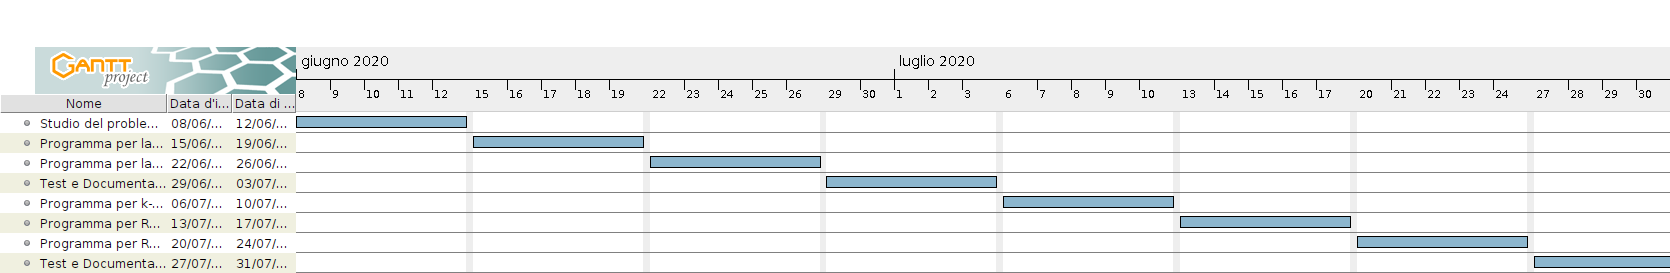
\includegraphics[scale=0.3]{./img/GanttVale.png}
    \captionof{figure}{Piano di Lavoro suddiviso per le 8 settimane previste dallo stage} \label{fig:ganttvale}
	 \end{center}
		